

\chapter{数值结果验证}

\section{基准算例}

为了验证\ProgramName 程序的临界计算及时空动力学计算功能,
本章使用业界常用的若干基准题对程序的结果进行验证。
临界计算的对比程序选用业内经典且广泛使用的Citation程序,
Citation程序是细网有限差分多群扩散临界计算程序。
\TODO

\subsection{静态IAEA PWR三维基准问题}
\label{sec:result.test.iaea}

IAEA 三维压水堆基准题是三维两群扩散基准题\cite{center1977benchmark},
由177个燃料组件构成,堆芯取$1/4$,
大小为170cm $\times$ 170cm $\times$ 380cm,
堆芯的几何结构见\floatref{fig:result.test.iaea},
堆芯中心为对称边界条件,外侧边界入流为0,外侧也可取等效边界条件
\begin{align}
  \frac{\partial \phi_g}{\partial n}=-\frac{0.4692}{D_g}\phi_g
\end{align}

各材料界面见\floatref{tab:result.test.iaea.mat},
裂变谱取$\chi_1=1$,$\chi_2=0$。

\begin{table}
\centering
\caption{\label{tab:result.test.iaea.mat}静态IAEA PWR 三维基准题材料截面}
\begin{tabular}{cccccc}
\toprule
材料 & 能群$g$ & $D_g/\mathrm{cm}$ & $\Sigma_{a,g}/\mathrm{cm}^{-1}$
    & $\nu\Sigma_{f,g}/n,\mathrm{cm}^{-1}$
    & $\Sigma_{s,1\rightarrow2}/\mathrm{cm}^{-1}$\\
\midrule
\multirow{2}{*}{M1} 
  & 1 & 1.5 & 0.01 & 0 & \multirow{2}{*}{0.02} \\
  & 2 & 0.4 & 0.08 & 0.135 &\\
\multirow{2}{*}{M2} 
  & 1 & 1.5 & 0.01 & 0 & \multirow{2}{*}{0.02} \\
  & 2 & 0.4 & 0.085 & 0.135 &\\
\multirow{2}{*}{M3} 
  & 1 & 1.5 & 0.01 & 0 & \multirow{2}{*}{0.02} \\
  & 2 & 0.4 & 0.13 & 0.135 &\\
\multirow{2}{*}{M4} 
  & 1 & 2.0 & 0 & 0 & \multirow{2}{*}{0.04} \\
  & 2 & 0.3 & 0.01 & 0 &\\
\multirow{2}{*}{M5} 
  & 1 & 2.0 & 0 & 0 & \multirow{2}{*}{0.04} \\
  & 2 & 0.3 & 0.055 & 0 &\\
\bottomrule
\end{tabular}
\end{table}

\begin{figure}
\centering
\begin{subfigure}{\textwidth}
\centering
\begin{tikzpicture}[scale=0.7, transform shape]
\def\lenscale{0.06}

\def\x#1{#1*\lenscale}
\def\zz#1{#1*\lenscale-8}
\def\z#1{#1*\lenscale}

\draw [very thick] (0,0) -- (\x{170},0) 
            -- (\x{170}, \zz{380}) -- (0, \zz{380});
\draw [loosely dashdotted] (0,0) -- (0, \zz{380});
\draw (0,\z{20}) -- (\x{150},\z{20}) -- (\x{150},\zz{360}) -- (0,\zz{360});
\draw (\x{10},\z{20}) -- (\x{10},\zz{380});
\draw [dashed] (\x{30},\zz{380}) -- (\x{30},\zz{280}) -- (\x{50},\zz{280}) -- (\x{50},\zz{380});
\draw (\x{70},\z{20}) -- (\x{70},\zz{380});
\draw (\x{90}, \z{20}) -- (\x{90},\zz{380});
\draw (\x{130},\z{20}) -- (\x{130},\zz{360});
\node at (\x{10},\z{80}) {\huge $\approx$};
\node at (\x{70},\z{80}) {\huge $\approx$};
\node at (\x{90},\z{80}) {\huge $\approx$};
\node at (\x{130},\z{80}) {\huge $\approx$};
\node at (\x{150},\z{80}) {\huge $\approx$};
\node at (\x{170},\z{80}) {\huge $\approx$};

\node [left] at (0,0) {\Large 0};
\node [left] at (0,\z{20}) {\Large 20};
\node [left] at (0,\zz{280}) {\Large 280};
\node [left] at (0,\zz{360}) {\Large 360};
\node [left] at (0,\zz{380}) {\Large 380};

\foreach \xp in {0, 10,30,50,70,90,130,150,170}
{
\node [above] at (\x{\xp},\zz{380}) {\Large \xp};
}

\node at (\x{160}, \zz{260}) {\Large M4};
\node at (\x{140}, \zz{260}) {\Large M1};
\node at (\x{110}, \zz{260}) {\Large M2};
\node at (\x{80}, \zz{260}) {\Large M3};
\node at (\x{40}, \zz{260}) {\Large M2};

\draw [-latex new, arrow head=3mm] (-1,\zz{260}) -- (\x{5}, \zz{260});
\node [left] at (-1, \zz{260}) {\Large M3};

%\draw [-latex new, arrow head=3mm] (-1,\zz{320}) -- (\x{40}, \zz{320});
%\node [left] at (-1, \zz{320}) {\Large Mp3};
\node at (\x{40}, \zz{320}) {\Large M3};

\node at (\x{80}, \zz{370}) {\Large M5};
\node at (\x{60}, \zz{370}) {\Large M4};
\node at (\x{40}, \zz{370}) {\Large M5};
\node at (\x{20}, \zz{370}) {\Large M4};

\draw [-latex new, arrow head=3mm] (-1,\zz{370}) -- (\x{5}, \zz{370});
\node [left] at (-1, \zz{370}) {\Large M5};

\node [above] at (-0.5,\zz{380}+0.5) {\Large cm};
\node [above] at (\x{170}+1,\zz{380}) {\Large cm};
\end{tikzpicture}
\caption{纵截面图}
\end{subfigure}
\begin{subfigure}{\textwidth}
\centering
\begin{tikzpicture}[scale=0.7, transform shape]
\def\lenscale{0.06}
\def\x#1{#1*\lenscale}

\draw [loosely dashdotted] (\x{170},0) -- (0,0) -- (0,\x{170});
%\draw [loosely dashdotted] (0,0) -- (\x{170},\x{170});

\draw (\x{10},0) -- (\x{10},\x{10}) -- (0,\x{10});

\draw (\x{70},0) -- (\x{70},\x{10}) -- (\x{90},\x{10}) -- (\x{90},0);
\draw (0,\x{70}) -- (\x{10},\x{70}) -- (\x{10},\x{90}) -- (0,\x{90});
\node [left] at (-1,\x{80}) {\Large M3};
\draw [-latex new, arrow head=3mm] (-1,\x{80}) -- (\x{5}, \x{80});
\node at (\x{80},\x{5}) {\Large M3};

\draw (\x{30},\x{30}) rectangle (\x{50},\x{50});
\node at (\x{40},\x{40}) {\Large M3};

\draw (0,\x{130}) -- (\x{30},\x{130}) -- (\x{30},\x{110})
           -- (\x{70},\x{110}) -- (\x{70},\x{70})
           -- (\x{110},\x{70}) -- (\x{110},\x{30})-- (\x{130},\x{30})
           -- (\x{130},0);
\node at (\x{40},\x{80}) {\Large M2};

\draw (\x{70},\x{70}) rectangle (\x{90},\x{90});
\node at (\x{80},\x{80}) {\Large M3};

\draw (0,\x{150}) -- (\x{50},\x{150}) -- (\x{50},\x{130})
           -- (\x{90},\x{130}) -- (\x{90},\x{110})
           -- (\x{110},\x{110})
           -- (\x{110},\x{90}) -- (\x{130},\x{90})-- (\x{130},\x{50})
           -- (\x{150},\x{50}) -- (\x{150},0);
\node at (\x{50},\x{120}) {\Large M1};

\draw [very thick] (0,\x{170}) -- (\x{70},\x{170}) -- (\x{70},\x{150})
           -- (\x{110},\x{150}) -- (\x{110},\x{130})
           -- (\x{130},\x{130})
           -- (\x{130},\x{110}) -- (\x{150},\x{110})-- (\x{150},\x{70})
           -- (\x{170},\x{70}) -- (\x{170},0);
\node at (\x{70},\x{140}) {\Large M4};

\foreach \xp in {0, 10,30,50,70,90,130,150,170}
{
\node [below] at (\x{\xp},0) {\Large \xp};
\node [left] at (0,\x{\xp}) {\Large \xp};
}

\node [below] at (\x{170}+1,0) {\Large cm};
\node [left] at (0, \x{170}+0.5) {\Large cm};

\draw [-latex new, arrow head=3mm](-1,\x{5}) -- (\x{5},\x{5});
\node [left] at (-1,\x{5}) {\Large M3};

\end{tikzpicture}
\caption{横截面图}
\end{subfigure}
\caption{\label{fig:result.test.iaea}静态IAEA PWR 三维基准题堆芯几何}
\end{figure}

\FloatBarrier
\subsection{动态TWIGL二维基准问题}
\label{sec:result.test.twigl}
TWIGL是二维两群扩散时空动力学基准题,
在1969年由Hageman和Yasinsky
于文献\onlinecite{hageman1969comparison}中提出\cite{gehin1992quasi},
堆芯取$1/4$,大小为80cm $\times$ 80cm,
堆芯的几何结构见\floatref{fig:result.test.twigl},
堆芯中心为对称边界条件,外侧边界入流为0。

各材料界面见\floatref{tab:result.test.twigl.mat},
裂变谱和缓发中子谱取$\chi_1=1$,$\chi_2=0$。
群速度为
\begin{align}
  \left\{
  \begin{aligned}
  v_1&=1.0\times10^7\mathrm{cm/s}\\
  v_2&=2.0\times10^5\mathrm{cm/s}
  \end{aligned}
  \right.
\end{align}
缓发中子为单组缓发中子
\begin{align}
  \left\{
  \begin{aligned}
  \beta&=0.0075\\
  \lambda&=0.08\mathrm{s}^{-1}
  \end{aligned}
  \right.
\end{align}
反应性引入方式
\begin{enumerate}
\item 阶跃引入:
\begin{align}
\Delta\Sigma_{a,2}&=-0.0035\mathrm{cm}^{-1} \quad t=0
\end{align}

\item 线性引入:
\begin{align}
\Sigma_{a,2}(t)&=\begin{cases}
    (1-0.11667t)\Sigma_{a,2}(0) & t\le 0.2\\
    0.97666\Sigma_{a,2}(0) & t > 0.2
  \end{cases}
\end{align}


\end{enumerate}

\begin{table}
\centering
\caption{\label{tab:result.test.twigl.mat}动态TWIGL二维基准题材料截面}
\begin{tabular}{cccccc}
\toprule
材料 & 能群$g$ & $D_g/\mathrm{cm}$ & $\Sigma_{a,g}/\mathrm{cm}^{-1}$
    & $\nu\Sigma_{f,g}/n,\mathrm{cm}^{-1}$
    & $\Sigma_{s,1\rightarrow2}/\mathrm{cm}^{-1}$\\
\midrule
\multirow{2}{*}{M1} 
  & 1 & 1.4 & 0.01 & 0.007 & \multirow{2}{*}{0.01} \\
  & 2 & 0.4 & 0.15 & 0.2 &\\
\multirow{2}{*}{M2} 
  & 1 & 1.4 & 0.01 & 0.007 & \multirow{2}{*}{0.01} \\
  & 2 & 0.4 & 0.15 & 0.2 &\\
\multirow{2}{*}{M3} 
  & 1 & 1.3 & 0.008 & 0.003 & \multirow{2}{*}{0.01} \\
  & 2 & 0.5 & 0.05 & 0.06 &\\
\bottomrule
\end{tabular}
\end{table}

\begin{figure}
\centering
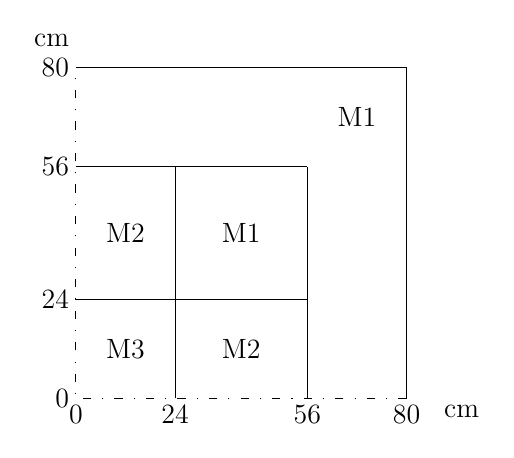
\begin{tikzpicture}[scale=0.7, transform shape]
\def\lenscale{0.075}
\def\x#1{#1*\lenscale}

\draw [loosely dashdotted] (\x{80},0) -- (0,0) -- (0,\x{80});

\draw (\x{24},0) -- (\x{24},\x{56});
\draw (0,\x{24}) -- (\x{56},\x{24});
\draw (\x{56},0) -- (\x{56},\x{56});
\draw (0,\x{56}) -- (\x{56},\x{56});
\draw (\x{80},0) -- (\x{80},\x{80});
\draw (0,\x{80}) -- (\x{80},\x{80});

\node at (\x{12},\x{12}) {\Large M3};
\node at (\x{40},\x{12}) {\Large M2};
\node at (\x{12},\x{40}) {\Large M2};
\node at (\x{40},\x{40}) {\Large M1};
\node at (\x{68},\x{68}) {\Large M1};

\foreach \xp in {0, 24, 56,80}
{
\node [below] at (\x{\xp},0) {\Large \xp};
\node [left] at (0,\x{\xp}) {\Large \xp};
}

\node [below] at (\x{80}+1,0) {\Large cm};
\node [left] at (0, \x{80}+0.5) {\Large cm};

\end{tikzpicture}
\caption{\label{fig:result.test.twigl}动态TWIGL二维基准题堆芯几何}
\end{figure}

\FloatBarrier
\subsection{动态LMW三维基准问题}

LMW(Langenbuch-Maurer-Werner)基准题\cite{langenbuch1977coarse,gehin1992quasi}是
三维两群扩散中子时空动力学基准题,
大小为$1/4$堆芯,几何尺寸110cm $\times$ 110cm $\times$ 200cm,
见\floatref{fig:result.test.lmw}。

\begin{figure}
\centering
\begin{subfigure}{.45\textwidth}
\hspace{-1.5cm}
\begin{tikzpicture}[scale=0.7, transform shape]
\def\lenscale{0.075}
\def\x#1{#1*\lenscale}

\draw [loosely dashdotted] (\x{110},0) -- (0,0) -- (0,\x{110});

\draw (\x{10},\x{0}) -- (\x{10},\x{10}) -- (\x{0},\x{10});
\draw (\x{50},\x{0}) -- (\x{50},\x{10}) -- (\x{70},\x{10}) -- (\x{70},\x{0});
\draw (\x{0},\x{50}) -- (\x{10},\x{50}) -- (\x{10},\x{70}) -- (\x{0},\x{70});
\node at (\x{30},\x{10}) {\Large M1};
\node at (\x{60},\x{5}) {\Large M2};
\node at (\x{5},\x{60}) {\Large M2};
\node at (\x{5},\x{5}) {\Large M2};

\draw (\x{30},\x{30}) rectangle (\x{50},\x{50});
\node at (\x{40},\x{40}) {\Large M2};

\draw (\x{70},\x{0}) -- (\x{70},\x{50}) -- (\x{50},\x{50})
      -- (\x{50},\x{70}) -- (\x{0},\x{70});
\node at (\x{60},\x{60}) {\Large M3};

\draw (\x{90},\x{0}) -- (\x{90},\x{70}) -- (\x{70},\x{70})
      -- (\x{70},\x{90}) -- (\x{0},\x{90});
\node at (\x{80},\x{80}) {\Large M4};

\draw (\x{110},\x{0}) -- (\x{110},\x{90}) -- (\x{90},\x{90})
      -- (\x{90},\x{110}) -- (\x{0},\x{110});

\foreach \xp in {0, 10,30,50,70,90,110}
{
\node [below] at (\x{\xp},0) {\Large \xp};
\node [left] at (0,\x{\xp}) {\Large \xp};
}

\node [below] at (\x{110}+1,0) {\Large cm};
\node [left] at (0, \x{110}+0.5) {\Large cm};

\draw [-latex new, arrow head=3mm] (-1.25,\x{50}) -- (\x{0},\x{60});
\draw [-latex new, arrow head=3mm] (-1.25,\x{50}) -- (\x{60},\x{10});
\node [left] at (-1.25,\x{50}) {\Large 第一组};

\draw [-latex new, arrow head=3mm] (-1.25,\x{20}) -- (\x{5},\x{10});
\draw [-latex new, arrow head=3mm] (-1.25,\x{20}) -- (\x{30},\x{40});
\node [left] at (-1.25,\x{20}) {\Large 第二组};

\end{tikzpicture}
\caption{横截面图}
\end{subfigure}
\\[1cm]
\begin{subfigure}{.45\textwidth}
\begin{tikzpicture}[scale=0.7, transform shape]
\def\lenscale{0.06}

\def\x#1{#1*\lenscale}
\def\zz#1{#1*\lenscale}
\def\z#1{#1*\lenscale}

\draw [very thick] (0,0) -- (\x{110},0) 
            -- (\x{110}, \zz{200}) -- (0, \zz{200});
\draw [loosely dashdotted] (0,0) -- (0, \zz{200});

\draw (0,\z{20}) -- (\x{90},\z{20}) -- (\x{90},\x{180}) -- (0,\zz{180});
\draw (\x{70},\x{20}) -- (\x{70},\x{180});

\node [left] at (0,0) {\Large 0};
\node [left] at (0,\z{20}) {\Large 20};
\node [left] at (0,\z{60}) {\Large 60};
\node [left] at (0,\z{100}) {\Large 100};
\node [left] at (0,\zz{180}) {\Large 180};
\node [left] at (0,\zz{200}) {\Large 200};

\node at (\x{30},\x{40}) {\Large M1};
\node at (\x{80},\x{100}) {\Large M3};
\node at (\x{100},\x{100}) {\Large M4};
\node at (\x{20},\x{190}) {\Large M4};
\node at (\x{40},\x{190}) {\Large M2};
\node at (\x{60},\x{190}) {\Large M2};
\draw [-latex new, arrow head=3mm] (-1,\x{190}) -- (\x{5},\x{190});
\node [left] at (-1,\x{190}) {\Large M2};

\draw [dashed] (\x{0},\x{100}) -- (\x{10},\x{100}) -- (\x{10},\x{200});
\draw (\x{10},\x{180}) -- (\x{10},\x{200});
\draw (\x{50},\x{200}) -- (\x{50},\x{100}) -- (\x{70},\x{100}) -- (\x{70},\x{200});
\draw [dashed] (\x{30},\x{180}) -- (\x{30},\x{200});

\node at (\x{60},\x{140}) {\Large M2};
\draw [-latex new, arrow head=3mm] (-1,\x{140}) -- (\x{5},\x{140});
\node [left] at (-1,\x{140}) {\Large M2};

\draw [-latex new, arrow head=3mm] (-1,\x{70}) -- (\x{5},\x{100});
\draw [-latex new, arrow head=3mm] (-1,\x{70}) -- (\x{60},\x{100});
\node [left] at (-1,\x{70}) {\Large 第一组};
\draw [-latex new, arrow head=3mm] (-1,\x{160}) -- (\x{5},\x{180});
\draw [-latex new, arrow head=3mm] (-1,\x{160}) -- (\x{40},\x{180});
\node [left] at (-1,\x{160}) {\Large 第二组};

\foreach \xp in {0,10,30,50,70,90,110}
{
\node [above] at (\x{\xp},\zz{200}) {\Large \xp};
}

\node at (-0.75,\zz{200}+0.75) {\Large cm};
\end{tikzpicture}
\caption{纵截面图(初始时控制棒位置)}
\end{subfigure}
\begin{subfigure}{.45\textwidth}
\begin{tikzpicture}[scale=0.7, transform shape]
\def\lenscale{0.06}

\def\x#1{#1*\lenscale}
\def\zz#1{#1*\lenscale}
\def\z#1{#1*\lenscale}

\draw [very thick] (0,0) -- (\x{110},0) 
            -- (\x{110}, \zz{200}) -- (0, \zz{200});
\draw [loosely dashdotted] (0,0) -- (0, \zz{200});

\draw (0,\z{20}) -- (\x{90},\z{20}) -- (\x{90},\x{180}) -- (0,\zz{180});
\draw (\x{70},\x{20}) -- (\x{70},\x{180});

\node [left] at (0,0) {\Large 0};
\node [left] at (0,\z{20}) {\Large 20};
\node [left] at (0,\z{60}) {\Large 60};
\node [left] at (0,\z{100}) {\Large 100};
\node [left] at (0,\zz{180}) {\Large 180};
\node [left] at (0,\zz{200}) {\Large 200};

\node at (\x{30},\x{40}) {\Large M1};
\node at (\x{80},\x{100}) {\Large M3};
\node at (\x{100},\x{100}) {\Large M4};
\node at (\x{20},\x{190}) {\Large M4};
\node at (\x{40},\x{190}) {\Large M2};
\node at (\x{60},\x{190}) {\Large M2};
\draw [-latex new, arrow head=3mm] (-1,\x{190}) -- (\x{5},\x{190});
\node [left] at (-1,\x{190}) {\Large M2};

\draw (\x{0},\x{60}) -- (\x{10},\x{60}) -- (\x{10},\x{200});
\draw [dashed] (\x{30},\x{200}) -- (\x{30},\x{60}) -- (\x{50},\x{60}) -- (\x{50},\x{200});
\draw (\x{50},\x{180}) -- (\x{50},\x{200});
\draw (\x{70},\x{180}) -- (\x{70},\x{200});

\draw [-latex new, arrow head=3mm] (-1,\x{30}) -- (\x{5},\x{60});
\draw [-latex new, arrow head=3mm] (-1,\x{30}) -- (\x{40},\x{60});
\node [left] at (-1,\x{30}) {\Large 第二组};
\draw [-latex new, arrow head=3mm] (-1,\x{160}) -- (\x{5},\x{180});
\draw [-latex new, arrow head=3mm] (-1,\x{160}) -- (\x{60},\x{180});
\node [left] at (-1,\x{160}) {\Large 第一组};

\node at (\x{40},\x{120}) {\Large M2};
\draw [-latex new, arrow head=3mm] (-1,\x{120}) -- (\x{5},\x{120});
\node [left] at (-1,\x{120}) {\Large M2};

\foreach \xp in {0,10,30,50,70,90,110}
{
\node [above] at (\x{\xp},\zz{200}) {\Large \xp};
}

\node at (-0.75,\zz{200}+0.75) {\Large cm};
\end{tikzpicture}
\caption{纵截面图(最终控制棒位置)}
\end{subfigure}
\caption{\label{fig:result.test.lmw}动态LMW三维基准题堆芯几何}
\end{figure}

\begin{table}
\centering
\caption{\label{tab:result.test.lmw.mat}动态LMW三维基准题材料截面}
\begin{tabular}{cccccc}
\toprule
材料 & 能群$g$ & $D_g/\mathrm{cm}$ & $\Sigma_{a,g}/\mathrm{cm}^{-1}$
    & $\nu\Sigma_{f,g}/n,\mathrm{cm}^{-1}$
    & $\Sigma_{s,1\rightarrow2}/\mathrm{cm}^{-1}$\\
\midrule
\multirow{2}{*}{M1} 
  & 1 & 1.423913 & 0.01040206 & 0.006477691 & \multirow{2}{*}{0.0175555} \\
  & 2 & 0.356306 & 0.08766217 & 0.1127328 &\\
\multirow{2}{*}{M2} 
  & 1 & 1.423913 & 0.01095206 & 0.006477691 & \multirow{2}{*}{0.0175555} \\
  & 2 & 0.356306 & 0.09146217 & 0.1127328 &\\
\multirow{2}{*}{M3} 
  & 1 & 1.425611 & 0.01099263 & 0.007503284 & \multirow{2}{*}{0.01717768} \\
  & 2 & 0.350574 & 0.09925634 & 0.1378004 &\\
\multirow{2}{*}{M4} 
  & 1 & 1.634227 & 0.002660573 & 0 & \multirow{2}{*}{0.02759693} \\
  & 2 & 0.264002 & 0.04936351 & 0 &\\
\bottomrule
\end{tabular}
\end{table}


算例包含两组控制棒,开始时第一组控制棒以3cm/s的速度拔出,
26.67s时停止。第二组控制棒从7.5s开始以同样的速度插入,47.5s时停止,
控制棒位置随时间变化见\floatref{fig:result.test.lmw.rob}。
\begin{figure}
\centering
\includegraphics[scale=0.9]{result-test-lmw-rob}
\caption{\label{fig:result.test.lmw.rob}LMW算例控制棒位置随时间变化图}
\end{figure}

裂变谱和缓发中子谱取$\chi_1=1$,$\chi_2=0$。
群速度为
\begin{align}
  \left\{
  \begin{aligned}
  v_1&=1.25\times10^7\mathrm{cm/s}\\
  v_2&=2.5\times10^5\mathrm{cm/s}
  \end{aligned}
  \right.
\end{align}
缓发中子有6组,见\floatref{tab:result.test.lmw.mat.c}。

\begin{table}
\centering
\caption{\label{tab:result.test.lmw.mat.c}动态LMW三维基准题缓发中子数据}
\begin{tabular}{ccc}
\toprule
缓发中子组 & 缓发中子份额$\beta_i$ & 衰变常数$\lambda_i/\mathrm{s}^{-1}$\\
\midrule
1 & 0.000247 & 0.0127\\
2 & 0.0013845 & 0.0317\\
3 & 0.001222 & 0.1150\\
4 & 0.0026455 & 0.3110\\
5 & 0.000832 & 1.400\\
6 & 0.000169 & 3.870\\
\bottomrule
\end{tabular}
\end{table}


\section{数值结果及验证}

在比较\ProgramName 的计算结果和参考结果之前,
先介绍本文使用的通量误差的计算方式。

对于临界问题,程序计算得到的通量分布结果的绝对值无意义,
有意义的是各网格上通量的相对大小关系,
所以一般都需要对结果进行归一化,
再比较归一化后的通量结果。
那么选择的归一化方法就会影响到计算结果的对比,
常见的归一化方式是总功率归一化和最大通量归一化,
但这两种方法都有各自的问题:
由于堆芯中通量分布在不同的网格上可相差数个量级,
如果按照堆芯总功率进行归一化,那么堆芯中部功率较高的部分对归一化系数影响很大,
高通量区域的误差会通过归一化系数转移到到低通量区域上;
同理使用最大通量归一化时,通量最高处的误差会影响到其他所有点的误差结果。
在常见的组件级通量统计中,这种问题并不明显,
但在细网结果的相对误差比较中,这种影响就被放大了。

为了减小高通量网格对归一化系数的影响,本文使用所有网格上的相对幅值的均值作为
归一化系数,即待验证的通量分布$\phi$和参考通量分布$\psi$见的相对归一化系数取为
\begin{align}
  \eta = \frac{\ \displaystyle\sum_{\bm{k},g}\frac{\phi_{\bm{k},g}}{\psi_{\bm{k},g}}\ }
              {\displaystyle\sum_{\bm{k},g}1}
\end{align}
其中$\bm{k}$为空间网格编号,
则归一化后的各网格的最大相对误差为
\begin{align}
  e_\mathrm{max} = \max_{\bm{k},g}
      \left|
        \frac{\phi_{\bm{k},g}}{\eta\cdot\psi_{\bm{k},g}} - 1
      \right|
\end{align}
本文以后提到的最大相对误差均是指上式所定义的最大相对误差,
而且为了更好地反映有实际意义的堆芯内的通量的相对误差,
一般把堆芯活性区以外的水反射层处通量极低的网格滤掉。

本文中如无特殊声明,计算环境均为
\begin{itemize}
\item CPU: 2$\times$ Intel Xeon CPU X5670 2.93GHz (双路服务器)
\item 内存:24GB
\item GPU:NVIDIA GeForce GTX TITAN,6GB显存
\item 操作系统:Windows 7 SP1 64位
\end{itemize}

\subsection{静态IAEA PWR三维基准题}

使用Citation的计算结果作为参考解,
通量收敛精度$\epsilon_\phi$取$10^{-6}$和$10^{-5}$,
对于5cm、2.5cm、2cm、1cm的$k_\mathrm{eff}$计算结果
见\floatref{tab:result.iaea.citation}。
以下对比中使用Citation通量收敛精度$\epsilon_\phi$取$10^{-6}$的
结果作为基准解,
并记$10^{-5}$精度的结果相对$10^{-6}$精度结果的通量最大相对偏差为$\epsilon_{5}$。
可见对于Citation,精度取$10^{-5}$时对于细网情况仍有较大误差。

\ProgramName 的通量收敛精度取$\epsilon'_\phi=10^{-5}$,
需要注意的是\ProgramName 和Citation的收敛精度计算方式不同,
计算结果见\floatref{tab:result.iaea.self},
其中$\max\epsilon_{\phi_{A,g}}$表示各组件通量的最大相对误差。
可见在该精度下\ProgramName 计算的$k_\mathrm{eff}$ 偏差小于$1\times10^{-5}$,
细网通量最大相对误差小于$4\times10^{-3}$,对于
粗网预求解方法(记为DM),通量最大相对误差小于$2.5\times10^{-3}$。
CG-SG DM方法1cm网格$1/8$堆芯的组件
通量相对偏差结果见\floatref{fig:result.iaea.aphitable},
其中$\phi_R$是\ProgramName 的计算结果,$\phi_C$是Citation的计算结果,
$\epsilon(\phi)$是两者的相对偏差。


\begin{sidewaystable}
\pdfrotate
\centering
\caption{静态IAEA PWR三维基准题Citation计算结果}
\label{tab:result.iaea.citation}
\begin{tabular}{cccccc}
\toprule
\multirow{2}{*}{网格尺寸/cm}
   & \multicolumn{2}{c}{$\epsilon_\phi=10^{-6}$}  
   & \multicolumn{2}{c}{$\epsilon_\phi=10^{-5}$}  & \multirow{2}{*}{$\epsilon_{5}$}\\
 & $k_\mathrm{eff}$ & 计算时间/s & $k_\mathrm{eff}$ & 计算时间/s 
 & \\
\midrule
5.0 & 1.0288101 &    5.2 & 1.0288101 &     4.2 & $1.0\times10^{-3}$\\
2.5 & 1.0290707 &    74.1 & 1.0290709 &   41.5 & $1.0\times10^{-3}$\\
2.0 & 1.0291338 &   497.9 & 1.0291338 &  149.0 & $2.1\times10^{-3}$\\
1.0 & 1.0292318 & 21437.0 & 1.0292313 & 2143.1 & $6.2\times10^{-3}$\\
\bottomrule
\end{tabular}
\\[1cm]
\caption{静态IAEA PWR三维基准题\ProgramName 计算结果及误差}
\label{tab:result.iaea.self}
\begin{tabular}{ccccccc}
\toprule
网格尺寸/cm & 求解算法 
        & 计算时间/s & $k_\mathrm{eff}$ 
        & $\epsilon_{k_\mathrm{eff}}$
        & $\max\epsilon_{\phi_{\bm{k},g}}$
        & $\max\epsilon_{\phi_{A,g}}$\\
\midrule
5.0 & CG-SG    &   1.701 & 1.0288096 & $5.4\times10^{-7}$ & $1.9\times10^{-3}$ & $1.5\times10^{-4}$\\
2.5 & CG-SG    &   5.210 & 1.0290717 & $9.7\times10^{-7}$ & $2.0\times10^{-3}$ & $1.5\times10^{-4}$\\
2.5 & CG-SG DM &   3.885 & 1.0290747 & $4.0\times10^{-6}$ & $1.0\times10^{-3}$ & $3.0\times10^{-4}$\\
2.0 & CG-SG    &   9.719 & 1.0291336 & $2.4\times10^{-7}$ & $1.5\times10^{-3}$ & $1.1\times10^{-4}$\\
1.0 & CG-SG    & 100.994 & 1.0292392 & $7.4\times10^{-6}$ & $3.3\times10^{-3}$ & $2.5\times10^{-4}$\\
1.0 & CG-SG DM &  40.794 & 1.0292418 & $1.0\times10^{-5}$ & $2.3\times10^{-3}$ & $2.6\times10^{-4}$\\
\bottomrule
\end{tabular}
\end{sidewaystable}


\begin{figure}
\centering
\subcaptionbox{快群}{
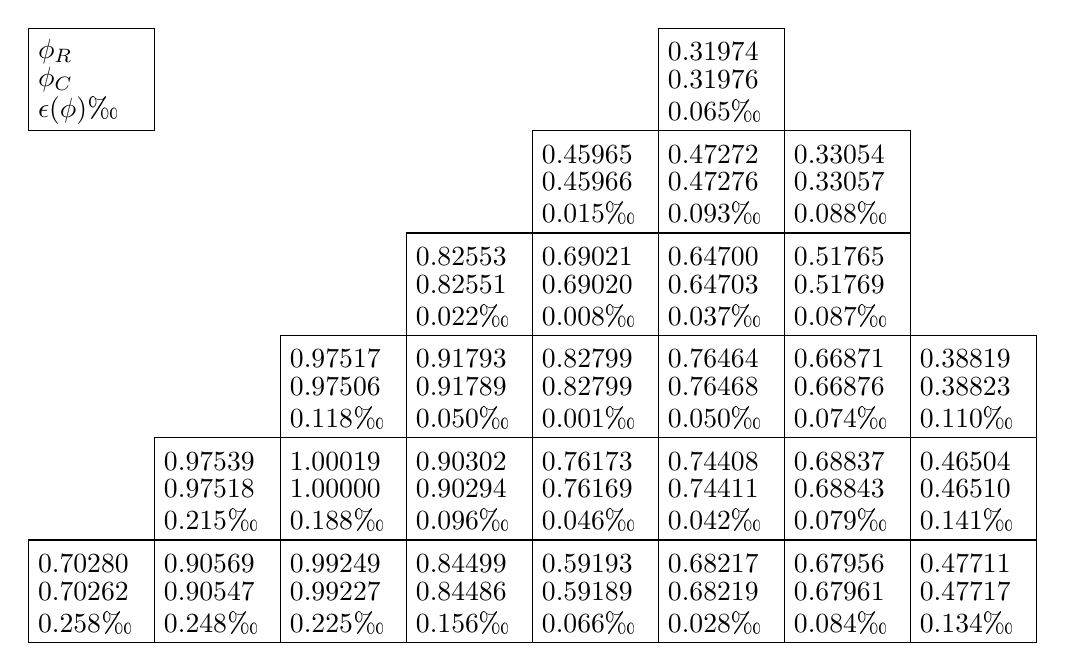
\begin{tikzpicture}
\def\di#1#2#3#4#5{
\def\boxx{1.6}
\def\boxy{1.3}
\draw (#1*\boxx, #2*\boxy) -- +(\boxx,0) -- +(\boxx,\boxy) -- +(0,\boxy) -- +(0,0);
\node [right] at (#1*\boxx,#2*\boxy+1) {#3};
\node [right]  at (#1*\boxx,#2*\boxy+0.65) {#4};
\node [right]  at (#1*\boxx,#2*\boxy+0.25) {#5\textperthousand};
}
\di{0}{5}{$\phi_R$}{$\phi_C$}{$\epsilon(\phi)$}
\di{0}{0}{0.70280}{0.70262}{0.258}
\di{1}{0}{0.90569}{0.90547}{0.248}
\di{1}{1}{0.97539}{0.97518}{0.215}
\di{2}{0}{0.99249}{0.99227}{0.225}
\di{2}{1}{1.00019}{1.00000}{0.188}
\di{2}{2}{0.97517}{0.97506}{0.118}
\di{3}{0}{0.84499}{0.84486}{0.156}
\di{3}{1}{0.90302}{0.90294}{0.096}
\di{3}{2}{0.91793}{0.91789}{0.050}
\di{3}{3}{0.82553}{0.82551}{0.022}
\di{4}{0}{0.59193}{0.59189}{0.066}
\di{4}{1}{0.76173}{0.76169}{0.046}
\di{4}{2}{0.82799}{0.82799}{0.001}
\di{4}{3}{0.69021}{0.69020}{0.008}
\di{4}{4}{0.45965}{0.45966}{0.015}
\di{5}{0}{0.68217}{0.68219}{0.028}
\di{5}{1}{0.74408}{0.74411}{0.042}
\di{5}{2}{0.76464}{0.76468}{0.050}
\di{5}{3}{0.64700}{0.64703}{0.037}
\di{5}{4}{0.47272}{0.47276}{0.093}
\di{5}{5}{0.31974}{0.31976}{0.065}
\di{6}{0}{0.67956}{0.67961}{0.084}
\di{6}{1}{0.68837}{0.68843}{0.079}
\di{6}{2}{0.66871}{0.66876}{0.074}
\di{6}{3}{0.51765}{0.51769}{0.087}
\di{6}{4}{0.33054}{0.33057}{0.088}
\di{7}{0}{0.47711}{0.47717}{0.134}
\di{7}{1}{0.46504}{0.46510}{0.141}
\di{7}{2}{0.38819}{0.38823}{0.110}
\end{tikzpicture}
}

\subcaptionbox{热群}{
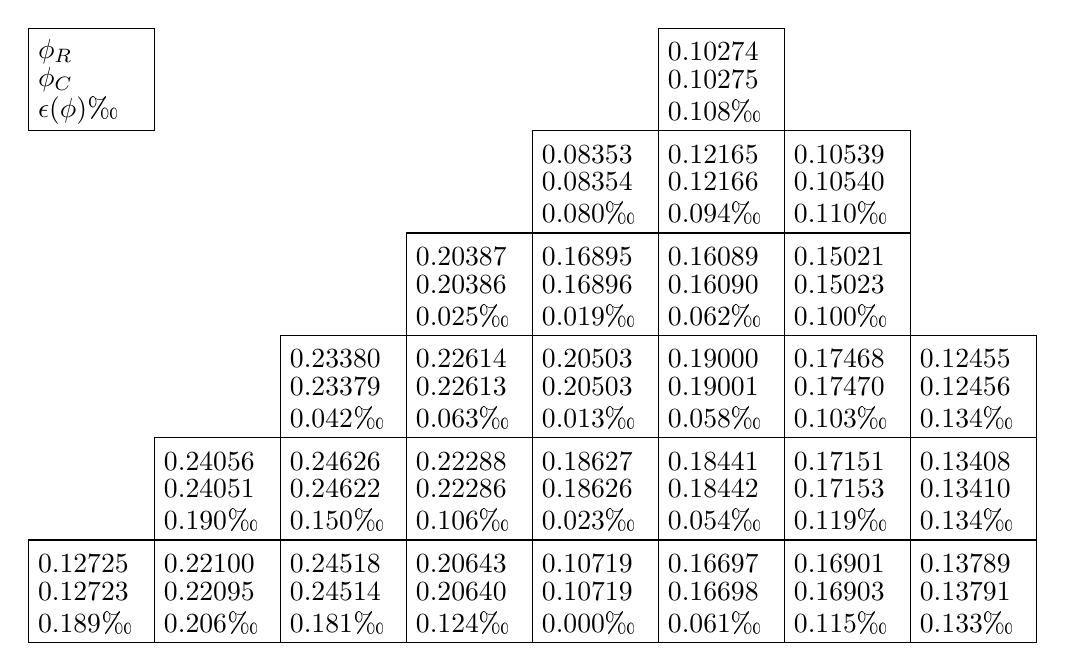
\begin{tikzpicture}
\def\di#1#2#3#4#5{
\def\boxx{1.6}
\def\boxy{1.3}
\draw (#1*\boxx, #2*\boxy) -- +(\boxx,0) -- +(\boxx,\boxy) -- +(0,\boxy) -- +(0,0);
\node [right] at (#1*\boxx,#2*\boxy+1) {#3};
\node [right] at (#1*\boxx,#2*\boxy+0.65) {#4};
\node [right] at (#1*\boxx,#2*\boxy+0.25) {#5\textperthousand};
}
\di{0}{5}{$\phi_R$}{$\phi_C$}{$\epsilon(\phi)$}
\di{0}{0}{0.12725}{0.12723}{0.189}
\di{1}{0}{0.22100}{0.22095}{0.206}
\di{1}{1}{0.24056}{0.24051}{0.190}
\di{2}{0}{0.24518}{0.24514}{0.181}
\di{2}{1}{0.24626}{0.24622}{0.150}
\di{2}{2}{0.23380}{0.23379}{0.042}
\di{3}{0}{0.20643}{0.20640}{0.124}
\di{3}{1}{0.22288}{0.22286}{0.106}
\di{3}{2}{0.22614}{0.22613}{0.063}
\di{3}{3}{0.20387}{0.20386}{0.025}
\di{4}{0}{0.10719}{0.10719}{0.000}
\di{4}{1}{0.18627}{0.18626}{0.023}
\di{4}{2}{0.20503}{0.20503}{0.013}
\di{4}{3}{0.16895}{0.16896}{0.019}
\di{4}{4}{0.08353}{0.08354}{0.080}
\di{5}{0}{0.16697}{0.16698}{0.061}
\di{5}{1}{0.18441}{0.18442}{0.054}
\di{5}{2}{0.19000}{0.19001}{0.058}
\di{5}{3}{0.16089}{0.16090}{0.062}
\di{5}{4}{0.12165}{0.12166}{0.094}
\di{5}{5}{0.10274}{0.10275}{0.108}
\di{6}{0}{0.16901}{0.16903}{0.115}
\di{6}{1}{0.17151}{0.17153}{0.119}
\di{6}{2}{0.17468}{0.17470}{0.103}
\di{6}{3}{0.15021}{0.15023}{0.100}
\di{6}{4}{0.10539}{0.10540}{0.110}
\di{7}{0}{0.13789}{0.13791}{0.133}
\di{7}{1}{0.13408}{0.13410}{0.134}
\di{7}{2}{0.12455}{0.12456}{0.134}
\end{tikzpicture}
}
\caption{\ProgramName 静态IAEA三维基准题1cm网格$1/8$堆芯组件通量相对偏差}
\label{fig:result.iaea.aphitable}
\end{figure}

\subsection{动态TWIGL二维基准问题}

动态TWIGL二维基准题的计算结果及对比见\floatref{tab:result.twigl.power-compare},
可见\ProgramName 和各种节块程序的结果符合的较好。

\begin{table}
\centering
\begin{minipage}{\textwidth}
\centering
\caption{动态TWIGL二维基准问题计算结果(堆芯相对功率)\label{tab:result.twigl.power-compare}}
\subcaptionbox{阶跃反应性基准题\label{tab:result.twigl.power-compare.1}}
{
\begin{tabular}{cccccc}
\toprule
系统时刻/s & QUANDRY\footnote{使用解析节块法,时间步长0.01s,
             数据来源\onlinecite{smith1979analytic,zhaowenbo}。}
         & NEM\footnote{使用节块展开法,网格8cm$\times$8cm,时间步长0.005s,
             数据来源\onlinecite{bandini1990three,zhaowenbo}。}
         & NGFMN-K\footnote{使用节块格林函数法,网格8cm$\times$8cm,计算方法DIRK(5,4)-E,
             计算精度1e-5,数据来源\onlinecite{zhaowenbo}。}
         & SPANDEX\footnote{使用变时间步节块展开法,网格4cm$\times$4cm,时间步长0.0001s,
             数据来源\onlinecite{aviles1993development,sutton1996diffusion}。}
         & \ProgramName \footnote{本文工作,细网有限差分法,
             网格划分1cm$\times$1cm,时间步长$0.01$s。}
         \\
\midrule
0.1 & 2.064 & 2.060 & 2.061 & 2.062 & 2.060 \\
0.2 & 2.076 & 2.078 & 2.079 & 2.079 & 2.079 \\
0.3 & 2.095 & 2.095 & 2.096 & 2.096 & 2.096 \\
0.4 & 2.112 & 2.113 & 2.114 & 2.114 & 2.114 \\
0.5 & 2.130 & 2.131 & 2.131 & 2.131 & 2.131 \\
\bottomrule
\end{tabular}
}
\\[1cm]
\subcaptionbox{线性反应性基准题\label{tab:result.twigl.power-compare.2}}
{
\begin{tabular}{cccccc}
\toprule
系统时刻/s & QUANDRY\footnote{时间步长0.005s,
             数据来源\onlinecite{smith1979analytic,zhaowenbo}。}
         & NEM\footnote{网格8cm$\times$8cm,时间步长0.005s,
             数据来源\onlinecite{bandini1990three,zhaowenbo}。}
         & NGFMN-K\footnote{网格8cm$\times$8cm,计算方法DIRK(5,4)-E,
             计算精度1e-5,数据来源\onlinecite{zhaowenbo}。}
         & SPANDEX\footnote{网格4cm$\times$4cm,时间步长0.0001s,
             数据来源\onlinecite{aviles1993development,sutton1996diffusion}。}
         & \ProgramName \footnote{网格划分1cm$\times$1cm,时间步长$0.005$s。}
         \\
\midrule
0.1 & 1.305 & 1.309 & 1.309 & 1.309 & 1.309 \\
0.2 & 1.954 & 1.962 & 1.960 & 1.960 & 1.962 \\
0.3 & 2.074 & 2.075 & 2.075 & 2.075 & 2.076 \\
0.4 & 2.092 & 2.092 & 2.092 & 2.092 & 2.093 \\
0.5 & 2.109 & 2.110 & 2.110 & 2.110 & 2.111 \\
\bottomrule
\end{tabular}
}
\end{minipage}
\end{table}


\subsection{动态LMW三维基准问题}

动态LMW三维基准题的计算结果及对比见\floatref{tab:result.lmw.power-compare}。

\begin{sidewaystable}
\pdfrotate
\centering
\begin{minipage}{0.8\textwidth}
\centering
\caption{动态LMW三维基准问题计算结果(堆芯相对功率)}
\label{tab:result.lmw.power-compare}
\begin{tabular}{ccccccc}
\toprule
系统时刻/s & SKETCH-N\footnote{使用基于非线性迭代策略的CMFD方法,网格10cm$\times$10cm$\times$5cm,时间步长0.25s,
             数据来源\onlinecite{zimin1998nodal}。}
         & PANTHER\footnote{使用基于非线性迭代策略的解析节块法,网格10cm$\times$10cm$\times$5cm,时间步长0.25s,
             数据来源\onlinecite{sutton1996diffusion}。}
         & NGFMN-K\footnote{使用节块格林函数法,网格10cm$\times$10cm$\times$5cm,计算方法DIRK(5,4)-E,
             计算精度1e-5,数据来源\onlinecite{zhaowenbo}。}
         & SPANDEX\footnote{使用变时间步节块展开法,网格5cm$\times$5cm$\times$2.5cm,计算精度5e-2,
             数据来源\onlinecite{aviles1993development,sutton1996diffusion}。}
         & NLSANMT\footnote{使用基于非线性迭代策略的CMFD方法,网格10cm$\times$10cm$\times$5cm,时间步长0.25s,
             数据来源\onlinecite{liaochengkui,zhaowenbo}。}
         & \ProgramName \footnote{本文工作,细网有限差分法,
             网格划分1cm$\times$1cm$\times$1cm,时间步长$1/12$s。} 
         \\
\midrule
10 & 1.338 & 1.347 & 1.341 & 1.341 & 1.339 & 1.341\\
20 & 1.705 & 1.726 & 1.720 & 1.713 & 1.706 & 1.705\\
30 & 1.369 & 1.382 & 1.381 & 1.373 & 1.368 & 1.362\\
40 & 0.809 & 1.813 & 0.814 & 0.809 & 0.808 & 0.804\\
50 & 0.502 & 0.505 & 0.504 & 0.503 & 0.502 & 0.501\\
60 & 0.385 & 0.387 & 0.387 & 0.386 & 0.385 & 0.385\\ 
\bottomrule
\end{tabular}
\end{minipage}
\end{sidewaystable}


\section{参数影响对比}
